\section{Naključne konstrukcije}
Cilj poglavja je generiranje Ramanujanovih grafov na računalniku. Uporabili bomo najbolj enostaven možen algoritem; generiramo naključen \(d\)-regularen graf in izračunamo njegovo spektralno vrzel. Če je dovolj velika je naš graf Ramanujanov, če pa je premajhna pa graf zavržemo in generiramo nov graf, dokler ne dobimo takega, ki ima dovolj veliko spektralno vrzel. Računanje lastne vrednosti grafa je zelo enostavno, si bomo pa bližje ogledali algoritem za učinkovito generiranje naključnih regularnih grafov.

Z dobljenim algoritmom si lahko ogledamo nekaj lastnosti grafov. Zanima nas velikost spektralne vrzeli v odvisnosti od števila vozlišč in delež Ramanujanov grafov. Če je ta delež dovolj velik je naš algoritem učinkovit in lahko enostavno generiramo Ramanujanove grafe. Velikost povprečne spektralne vrzeli pa nam pove, kako daleč stran je poljuben graf od tega, da je Ramanujanov; imajo sicer zanimive matematične lastnosti, v praksi bi se pa morda kdaj zadovoljili že z grafom, ki je ``približno'' Ramanujanov.

\subsection{Algoritmi za generiranje regularnih grafov}
Generiranje regularnih grafov je netrivialen problem. Težava pri večini pristopov je, da ne moremo povezav dodajati iterativno in imeti zagotovljeno, da na koncu dobimo regularen graf. Oglejmo si to na enostavnem primeru.

\begin{primer}
    Za primer bomo poskusili generirati \(2\)-regularen graf na \(4\) vozliščih. Tak graf seveda obstaja, na primer cikel \(C_4\). Naš algoritem bo sledeč: izberemo naključni dve vozlišči, ki imata stopnjo manjšo od \(2\) in ju povežemo. To ponavljamo, dokler ne dobimo grafa, ki je \(2\)-regularen.

    Začnemo s praznim grafom, ki ima vozlišča \(\{1, 2, 3, 4\}\). Izberemo naključni dve vozlišči, recimo \(1\) in \(2\), in ju povežemo. Nato izberemo vozlišči \(2\) in \(3\) in ju povežemo, za tem pa še \(3\) in \(1\) in ju povežemo. Sedaj imamo \(3\) vozlišča stopnje \(2\) in enega stopnje \(0\). Ob vsaki točki smo izbrali vozlišči, ki imata stopnjo manjšo od \(2\), algoritem pa se ne more zaključiti, saj smo prišli do točke, saj vozlišča \(4\) ne moremo povezati z nobenim vozliščem, ki ima stopnjo manjšo od \(2\).
\end{primer}

V tem primeru je bil problem, da ne moremo povezati vozlišča s samim seboj, lahko pa bi se zgodilo tudi, da imamo dva vozlišča stopnje \(d-1\), ki pa ju ne moremo povezati, saj sta že povezani. Obstaja enostaven način da rešimo to težavo: če algoritma ne moremo zaključiti graf zavržemo in začnemo znova. Z malo optimizacije nas to prinese do naslednjega algoritma\cite{kim-vu-regularni}.

\algnewcommand\algorithmicto{\textbf{to}}
\algnewcommand\algorithmicin{\textbf{in}}
\algnewcommand\algorithmicforeach{\textbf{for each}}
\algrenewtext{For}[3]{\algorithmicfor\ #1 $\gets$ #2\ \algorithmicto\ #3\ \algorithmicdo}
\algdef{S}[FOR]{ForEach}[2]{\algorithmicforeach\ #1\ \algorithmicin\ #2\ \algorithmicdo}
Za vse pristope bomo uporabljali funkcijo, ki ponavlja klice na naš algoritem, dokler ne dobimo regularnega grafa.
\begin{algorithm}[ht]
    \caption{Generiranje naključnih regularnih grafov}
    \label{enakomerno-nakljucni-pocasi}
    \raggedright
    \textbf{Vhod:} Števili \(n, d \in n, d \in \mathbb N\). \\
    \textbf{Izhod:} Sosednostna matrika \(A\) \(d\)-regularnega grafa na \(n\) vozliščih.
    \begin{algorithmic}[1]
        \Function{generiraj}{$n$, $d$}
        \While{True}
        \State \(A \gets \Call{generiraj-pomozno}{n, d}\)
        \If{\Call{je-regularen-graf}{$A$, $d$}}
        \State \Return $A$
        \EndIf
        \EndWhile
        \EndFunction
    \end{algorithmic}
\end{algorithm}

\begin{algorithm}[ht]
    \caption{Generiranje naključnih regularnih grafov}
    \label{enakomerno-nakljucni-pocasi}
    \raggedright
    \textbf{Vhod:} Števili \(n, d \in n, d \in \mathbb N\). \\
    \textbf{Izhod:} Sosednostna matrika \(A\) \(d\)-regularnega grafa na \(n\) vozliščih.
    \begin{algorithmic}[1]
        \Function{generiraj-pomozno}{$n$, $d$}
        \For{$i$}{$0$}{$n-1$}
        \For{$j$}{$0$}{$d-1$}
        \State \(krajisce[i\cdot n + j] \gets i\) \Comment{Ustvarimo \(d\) kopij vsakega vozlišča.}
        \EndFor
        \EndFor
        \State \(krajisce' \gets \Call{shuffle}{krajisce}\)
        \State \(A \gets\) ničelna matrika velikosti \(n \times n\)
        \For{$i$}{$0$}{$n\cdot d - 1$}
        \State \(A_{krajisce[i], krajisce'[i]} \gets 1\)
        \State \(A_{krajisce'[i], krajisce[i]} \gets 1\)
        \EndFor
        \State \Return $A$
        \EndFunction
    \end{algorithmic}
\end{algorithm}

Algoritem je sicer pravilen, vendar pa je zelo počasen. Velikokrat se zgodi, da moremo ponovno generirati graf, še posebaj za velike \(d\), kar ga naredi neuporabnega za generiranje večjih grafov. Izkaže se, da je verjetnost generiranja regularnega grafa \(O(e^{-\frac{d^2}{4}})\), kar se zelo hitro približuje \(0\) ko povečujemo \(d\). Algoritem postane nepraktičen že, če želimo generirati \(10\) regularne grafe. Obstajajo algoritmi, ki imajo polinomsko časovno zahtevnost, vendar so še vedno počasni in zahtevni za implementirati. Lahko si pa olajšamo delo tako, da grafov ne generiramo enakomerno naključno\cite{STEGER_WORMALD_1999}.

\begin{algorithm}[ht]
    \caption{Hitro generiranje naključnih regularnih grafov}
    \label{enakomerno-nakljucni-hitro}
    \raggedright
    \textbf{Vhod:} Števili \(n, d \in n, d \in \mathbb N\). \\
    \textbf{Izhod:} Sosednostna matrika \(A\) \(d\)-regularnega grafa na \(n\) vozliščih.
    \begin{algorithmic}[1]
        \Function{ustrezen-par}{$i$, $j$, $pari$, $V$}
        \State \(i'\) tak, da \(i\in V[i']\)
        \State \(j'\) tak, da \(j\in V[j']\)
        \If{\(i' = j'\)}
        \State \Return False \Comment{Povezati želimo vozlišče s seboj.}
        \EndIf
        \If{\((i', j') \in pari\)}
        \State \Return False \Comment{Povezava že obstaja.}
        \EndIf
        \State \Return True
        \EndFunction
        \Function{generiraj-pomozno}{$n$, $d$}
        \State \(U = \{1, 2, \ldots, nd\}\) \Comment{Točke, ki še nimajo para}
        \For {$i$}{$0$}{$n-1$}
        \For {$j$}{$0$}{$d-1$}
        \State \(V[i][j] \gets i\cdot n + j\) \Comment{Ustvarimo \(d\) elementov za vsako vozlišče.}
        \EndFor
        \EndFor
        \State \(pari \gets []\)
        \While{\(\exists i,j \in U.\, \Call{ustrezen-par}{i, j, pari, V}\)}
        \State \(i\gets \Call{nakljucno-izberi}{U}\)
        \State \(j\gets \Call{nakljucno-izberi}{U}\)
        \If {\(\Call{ustrezen-par}{i, j}\)}
        \State Dodaj par \((i, j)\) v \(pari\)
        \State Izbriši \(i\) in \(j\) iz \(U\)
        \EndIf
        \EndWhile
        \State \(A \gets\) ničelna matrika velikosti \(n \times n\)
        \ForEach{$(i, j)$}{$pari$}
        \State{\(i'\) tak, da \(i\in V[i']\)}
        \State{\(j'\) tak, da \(j\in V[j']\)}
        \State \(A_{i', j'} \gets 1\)
        \State \(A_{j', i'} \gets 1\)
        \EndFor
        \State \Return $A$
        \EndFunction
    \end{algorithmic}
\end{algorithm}

Omenimo še bolj enostaven, naiven pristop za generiranje regularnih grafov. Tu je implementacija zelo enostavna in program dela razmeroma hitro, je pa daleč stran od enakomerne porazdelitve.

\begin{algorithm}[ht]
    \caption{Enostavno generiranje naključnih regularnih grafov}
    \label{enakomerno-nakljucni-hitro}
    \raggedright
    \textbf{Vhod:} Števili \(n, d \in n, d \in \mathbb N\). \\
    \textbf{Izhod:} Sosednostna matrika \(A\) \(d\)-regularnega grafa na \(n\) vozliščih.
    \begin{algorithmic}[1]
        \Function{generiraj-pomozno}{$n$, $d$}
        \State \(A \gets\) ničelna matrika velikosti \(n \times n\)
        \For {$i$}{$0$}{$n-1$}
        \State \(V \gets \) množica vozlišč, stopnje manj od \(d\), ki niso povezana z \(i\)
        \State \(d' \gets \Call{Stopnja}(i)\)
        \If {\(\abs{V} < d-d'\)}
        \State \Return \(A\)
        \EndIf
        \State \(V' \gets \) naključnih \(d-d'\) vozlišč iz \(V\)
        \State Dodamo povezave med \(i\) in vozlišči iz \(V'\) v \(A\)
        \EndFor
        \State \Return $A$
        \EndFunction
    \end{algorithmic}
\end{algorithm}

\begin{figure}[h!]
    \centering
    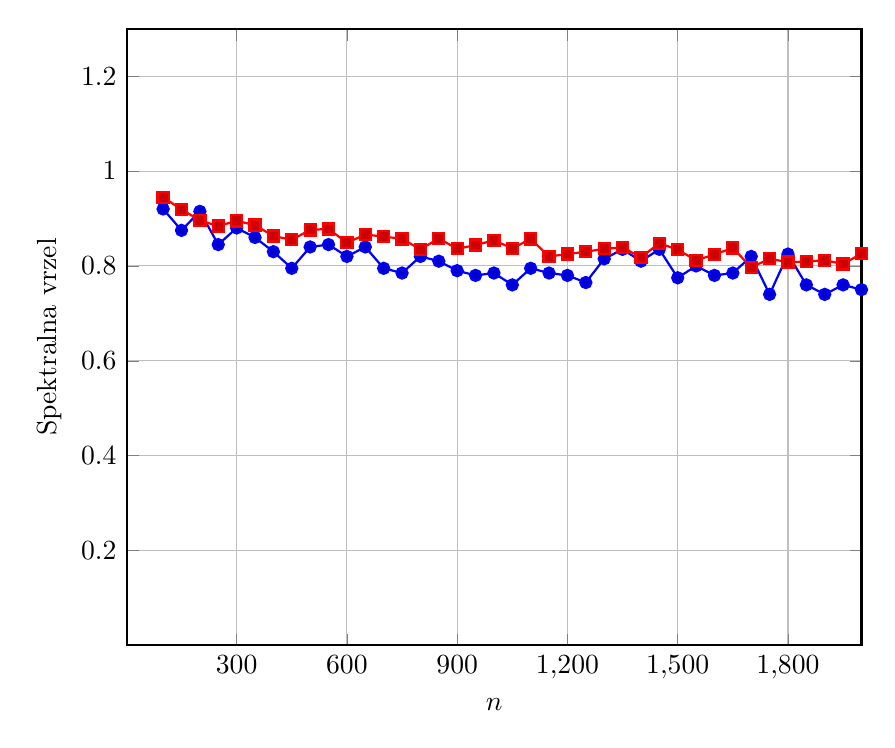
\begin{tikzpicture}
        \begin{axis}[
                xlabel={$n$},
                width=0.9\textwidth,
                ylabel={Spektralna vrzel},
                grid=major,
                ymin=0, ymax=1.3,
                xmin=1, xmax=2000,
                xtick={0,300,...,2000},
                ytick={0.2,0.4,0.6,0.8,1,1.2},
                thick
            ]
            \addplot coordinates {
                    (100, 0.92)
                    (150, 0.875)
                    (200, 0.915)
                    (250, 0.845)
                    (300, 0.88)
                    (350, 0.86)
                    (400, 0.83)
                    (450, 0.795)
                    (500, 0.84)
                    (550, 0.845)
                    (600, 0.82)
                    (650, 0.84)
                    (700, 0.795)
                    (750, 0.785)
                    (800, 0.82)
                    (850, 0.81)
                    (900, 0.79)
                    (950, 0.78)
                    (1000, 0.785)
                    (1050, 0.76)
                    (1100, 0.795)
                    (1150, 0.785)
                    (1200, 0.78)
                    (1250, 0.765)
                    (1300, 0.815)
                    (1350, 0.835)
                    (1400, 0.81)
                    (1450, 0.835)
                    (1500, 0.775)
                    (1550, 0.8)
                    (1600, 0.78)
                    (1650, 0.785)
                    (1700, 0.82)
                    (1750, 0.74)
                    (1800, 0.825)
                    (1850, 0.76)
                    (1900, 0.74)
                    (1950, 0.76)
                    (2000, 0.75)
                };
            \addplot coordinates {
                    (100, 0.945)
                    (150, 0.919)
                    (200, 0.896)
                    (250, 0.884)
                    (300, 0.895)
                    (350, 0.886)
                    (400, 0.863)
                    (450, 0.855)
                    (500, 0.876)
                    (550, 0.878)
                    (600, 0.849)
                    (650, 0.866)
                    (700, 0.862)
                    (750, 0.857)
                    (800, 0.835)
                    (850, 0.858)
                    (900, 0.836)
                    (950, 0.844)
                    (1000, 0.854)
                    (1050, 0.837)
                    (1100, 0.857)
                    (1150, 0.82)
                    (1200, 0.825)
                    (1250, 0.83)
                    (1300, 0.836)
                    (1350, 0.839)
                    (1400, 0.818)
                    (1450, 0.848)
                    (1500, 0.834)
                    (1550, 0.812)
                    (1600, 0.824)
                    (1650, 0.838)
                    (1700, 0.797)
                    (1750, 0.815)
                    (1800, 0.808)
                    (1850, 0.809)
                    (1900, 0.812)
                    (1950, 0.804)
                    (2000, 0.826)
                };
        \end{axis}
    \end{tikzpicture}
    \caption{Graf proporcije Ramanujanovih grafov od 1 do 300}
\end{figure}

\begin{figure}[h!]
    \centering
    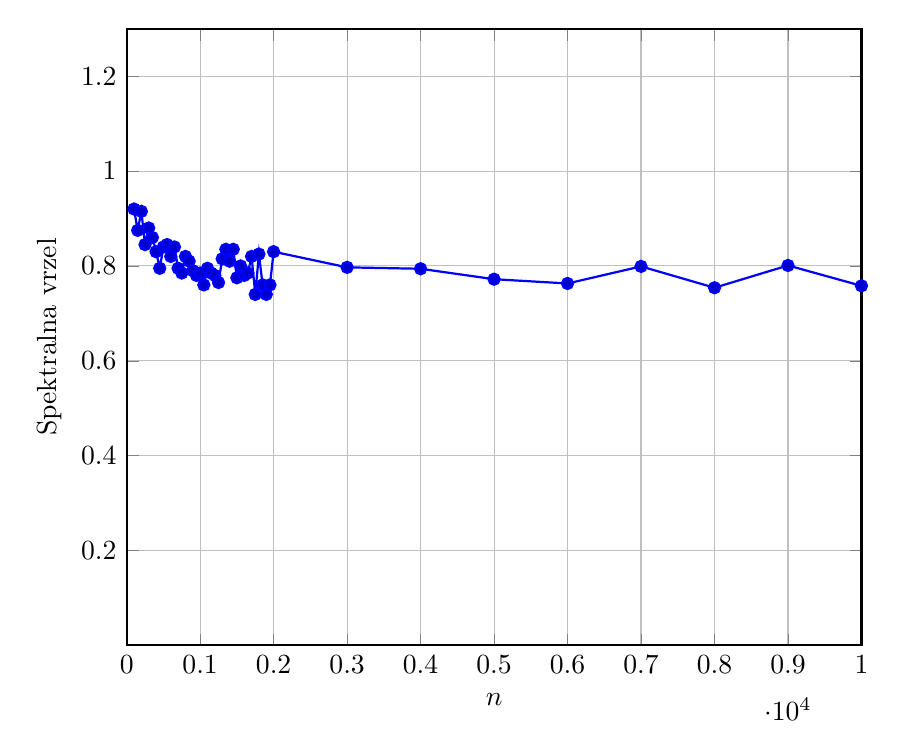
\begin{tikzpicture}
        \begin{axis}[
                xlabel={$n$},
                width=0.9\textwidth,
                ylabel={Spektralna vrzel},
                grid=major,
                ymin=0, ymax=1.3,
                xmin=1, xmax=10000,
                xtick={0,1000,...,10000},
                ytick={0.2,0.4,0.6,0.8,1,1.2},
                thick
            ]
            \addplot coordinates {
                    (100, 0.92)
                    (150, 0.875)
                    (200, 0.915)
                    (250, 0.845)
                    (300, 0.88)
                    (350, 0.86)
                    (400, 0.83)
                    (450, 0.795)
                    (500, 0.84)
                    (550, 0.845)
                    (600, 0.82)
                    (650, 0.84)
                    (700, 0.795)
                    (750, 0.785)
                    (800, 0.82)
                    (850, 0.81)
                    (900, 0.79)
                    (950, 0.78)
                    (1000, 0.785)
                    (1050, 0.76)
                    (1100, 0.795)
                    (1150, 0.785)
                    (1200, 0.78)
                    (1250, 0.765)
                    (1300, 0.815)
                    (1350, 0.835)
                    (1400, 0.81)
                    (1450, 0.835)
                    (1500, 0.775)
                    (1550, 0.8)
                    (1600, 0.78)
                    (1650, 0.785)
                    (1700, 0.82)
                    (1750, 0.74)
                    (1800, 0.825)
                    (1850, 0.76)
                    (1900, 0.74)
                    (1950, 0.76)
                    (2000, 0.83)
                    (3000, 0.797)
                    (4000, 0.794)
                    (5000, 0.772)
                    (6000, 0.763)
                    (7000, 0.799)
                    (8000, 0.754)
                    (9000, 0.801)
                    (10000, 0.758)
                };
        \end{axis}
    \end{tikzpicture}
    \caption{Graf proporcije Ramanujanovih grafov od 1000 do 10000}
\end{figure}

\begin{figure}[h!]
    \centering
    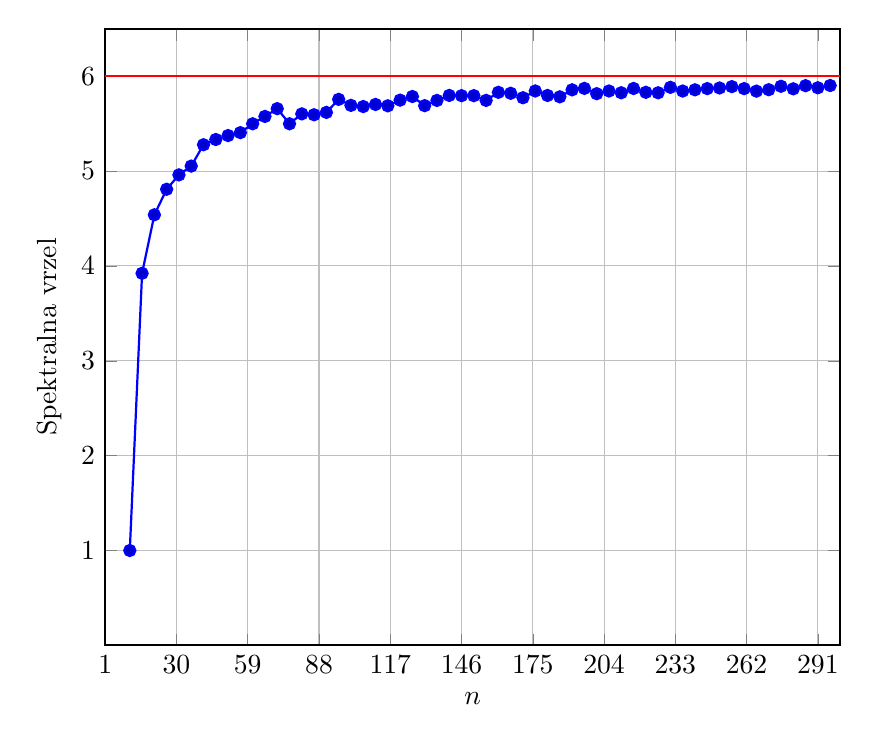
\begin{tikzpicture}
        \begin{axis}[
                xlabel={$n$},
                width=0.9\textwidth,
                ylabel={Spektralna vrzel},
                grid=major,
                ymin=0, ymax=6.5,
                xmin=1, xmax=300,
                xtick={1,30,...,300},
                ytick={1,2,3,4,5,6},
                thick
            ]
            \addplot coordinates {
                    (11, 1.000000000000002)
                    (16, 3.9222400439343685)
                    (21, 4.538860013159836)
                    (26, 4.808216830193524)
                    (31, 4.959790573039687)
                    (36, 5.052688498284467)
                    (41, 5.277523254626809)
                    (46, 5.332807138620655)
                    (51, 5.37442486437986)
                    (56, 5.405097185918946)
                    (61, 5.498571934186495)
                    (66, 5.575938409277276)
                    (71, 5.657944175537072)
                    (76, 5.498418778423789)
                    (81, 5.602860389811621)
                    (86, 5.593469989602875)
                    (91, 5.6184462225220955)
                    (96, 5.755892359656839)
                    (101, 5.692360968966922)
                    (106, 5.680076900644869)
                    (111, 5.702246521366402)
                    (116, 5.687849569151763)
                    (121, 5.7477099188934355)
                    (126, 5.786041727310356)
                    (131, 5.689452187703263)
                    (136, 5.744546954992545)
                    (141, 5.797192510119292)
                    (146, 5.794721314474317)
                    (151, 5.794856354446884)
                    (156, 5.7450428693297475)
                    (161, 5.830087183980121)
                    (166, 5.819987775195498)
                    (171, 5.773037906395612)
                    (176, 5.8442881137227465)
                    (181, 5.796921259614794)
                    (186, 5.7826092969682374)
                    (191, 5.856437633170694)
                    (196, 5.871746814293452)
                    (201, 5.815647264915688)
                    (206, 5.844111155403364)
                    (211, 5.82553111614388)
                    (216, 5.870565933769311)
                    (221, 5.830291882849532)
                    (226, 5.825318465358029)
                    (231, 5.8827281797714175)
                    (236, 5.84361148217756)
                    (241, 5.856540765886825)
                    (246, 5.869304300978469)
                    (251, 5.8758368544626185)
                    (256, 5.890130266065601)
                    (261, 5.8691466815061935)
                    (266, 5.842566144716664)
                    (271, 5.857769806232399)
                    (276, 5.893678696498535)
                    (281, 5.866955967785748)
                    (286, 5.89999683489138)
                    (291, 5.878019228343736)
                    (296, 5.901828771475102)
                };
            \addplot[red, thick] coordinates {(0, 6) (300, 6)};
        \end{axis}
    \end{tikzpicture}
    \caption{Graf spektralnih vrzeli za \(n\) od 1 do 300}
\end{figure}

